\documentclass[12pt]{article}
\usepackage[margin=2.5cm]{geometry}
\usepackage{enumerate}
\usepackage{amsfonts}
\usepackage{amsmath}
\usepackage{fancyhdr}
\usepackage{amsmath}
\usepackage{amssymb}
\usepackage{amsthm}
\usepackage{mdframed}
\usepackage{graphicx}
\usepackage{subcaption}
\usepackage{adjustbox}
\usepackage{listings}
\usepackage{xcolor}
\usepackage{soul}
\usepackage{booktabs}
\usepackage[utf]{kotex}
\usepackage{hyperref}

\definecolor{codegreen}{rgb}{0,0.6,0}
\definecolor{codegray}{rgb}{0.5,0.5,0.5}
\definecolor{codepurple}{rgb}{0.58,0,0.82}
\definecolor{backcolour}{rgb}{0.95,0.95,0.92}

\lstdefinestyle{mystyle}{
    backgroundcolor=\color{backcolour},
    commentstyle=\color{codegreen},
    keywordstyle=\color{magenta},
    numberstyle=\tiny\color{codegray},
    stringstyle=\color{codepurple},
    basicstyle=\ttfamily\footnotesize,
    breakatwhitespace=false,
    breaklines=true,
    captionpos=b,
    keepspaces=true,
    numbers=left,
    numbersep=5pt,
    showspaces=false,
    showstringspaces=false,
    showtabs=false,
    tabsize=1
}

\lstset{style=mystyle}

\pagestyle{fancy}
\renewcommand{\headrulewidth}{0.4pt}
\lhead{CSC 373}
\rhead{Worksheet 5 Solution}

\begin{document}
\title{CSC373 Worksheet 5 Solution}
\maketitle

\bigskip

\begin{enumerate}[1.]
    \item

    \bigskip

    \begin{proof}

    Assume that a flow network $G = (V,E)$ violates the assumption that the
    network contains a path $s \rightsquigarrow v \rightsquigarrow t$ for all
    vertices $v \in V$. Let $u$ be a vertex for which there is no path $s \rightsquigarrow u \rightsquigarrow t$.

    \bigskip

    I must show such that there is no flow at vertex $u$. That is, there exists a
    maximum flow $f$ in $G$ such that $f(u,v) = f(v,u) = 0$ for all vertices $v \in V$.

    \bigskip

    Assume for the sake of contradiction that there is some vertex $u$ with flow $f$.
    That is, there exists some vertices $v \in V$ such that $f(u,v) > 0$ or $f(v,u) > 0$.

    \bigskip

    I see that three cases follows, and I will prove each separately.

    \bigskip

    \begin{enumerate}[1.]
        \item \textbf{Cases 1:} $f(u,v) = 0$ and $f(v,u) > 0$

        \bigskip

        Here, assume that $f(u,v) = 0$ for all $v \in V$ and $f(v,u) > 0$ for some $v \in V$.

        \bigskip

        Then, we can write $\sum\limits_{v \in V} f(u,v) = 0$ and $\sum\limits_{v \in V} f(v,u) > 0$

        \bigskip

        But this violates the flow conservation property (i.e $\sum\limits_{v \in V} f(u,v) = \sum\limits_{v \in V} f(v,u)$)

        \bigskip

        Thus, by proof by contradiction, $f(u,v) = 0$ and $f(v,u) = 0$ for all $v \in V$ and
        all $u \in V$ with no path $s \rightsquigarrow u \rightsquigarrow t$.

        \bigskip

        \item \textbf{Cases 2:} $f(u,v) > 0$ and $f(v,u) = 0$

        \bigskip

        Here, assume that $f(u,v) > 0$ for some $v \in V$ and $f(v,u) = 0$ for all $v \in V$.

        \bigskip

        Then, by similar work as case 1, the same result follows.

        \bigskip

        \item \textbf{Cases 3:} $f(u,v) > 0$ and $f(v,u) > 0$

        \bigskip

        Here, assume that $f(u,v) > 0$ and $f(v,u) > 0$ for some $v \in V$.

        \bigskip

        Since $s \rightsquigarrow v \rightsquigarrow t$ and $u$ is connected by some vertices $v$,
        we can write $s \rightsquigarrow u \rightsquigarrow t$.

        \bigskip

        Then, this violates the fact in header that the vertex $u$ has no path $s \rightsquigarrow u \rightsquigarrow t$.

        \bigskip

        Thus, by proof by contradiction, $f(u,v) = 0$ and $f(v,u) = 0$ for all $v \in V$ and
        all $u \in V$ with no path $s \rightsquigarrow u \rightsquigarrow t$.

    \end{enumerate}

    \end{proof}

    \bigskip

    % \underline{\textbf{Rough Works:}}

    % \bigskip

    % Assume that a flow network $G = (V,E)$ violates the assumption that the
    % network contains a path $s \rightsquigarrow v \rightsquigarrow t$ for all
    % vertices $v \in V$. Let $u$ be a vertex for which there is no path $s \rightsquigarrow u \rightsquigarrow t$.

    % \bigskip

    % I must show such that there is no flow at vertex $u$. That is, there exists a
    % maximum flow $f$ in $G$ such that $f(u,v) = f(v,u) = 0$ for all vertices $v \in V$.

    % \bigskip

    % Assume for the sake of contradiction that there is some vertex $u$ with flow $f$.
    % That is, there exists some vertices $v \in V$ such that $f(u,v) > 0$ or $f(v,u) > 0$.

    % \bigskip

    % I see that three cases follows, and I will prove each separately.

    % \bigskip

    % \begin{enumerate}[1.]
    %     \item \textbf{Cases 1:} $f(u,v) = 0$ and $f(v,u) > 0$

    %     \bigskip

    %     Here, assume that $f(u,v) = 0$ for all $v \in V$ and $f(v,u) > 0$ for some $v \in V$.

    %     \bigskip

    %     \begin{itemize}
    %         \item Show that $\sum\limits_{v \in V} f(u,v) = 0$ and $\sum\limits_{v \in V} f(v,u) > 0$

    %         \begin{mdframed}
    %         Then, we can write $\sum\limits_{v \in V} f(u,v) = 0$ and $\sum\limits_{v \in V} f(v,u) > 0$
    %         \end{mdframed}

    %         \item Show that this violates flow conservation [contradiction]

    %         \begin{mdframed}
    %         But this violates the flow conservation property (i.e $\sum\limits_{v \in V} f(u,v) = \sum\limits_{v \in V} f(v,u)$)
    %         \end{mdframed}

    %         \item Conclude that $f(u,v) = 0$ and $f(v,u) = 0$

    %         \begin{mdframed}
    %         Thus, by proof by contradiction, $f(u,v) = 0$ and $f(v,u) = 0$ for all $v \in V$ and
    %         all $u \in V$ with no path $s \rightsquigarrow u \rightsquigarrow t$.
    %         \end{mdframed}
    %     \end{itemize}

    %     \begin{mdframed}
    %     Here, assume that $f(u,v) = 0$ for all $v \in V$ and $f(v,u) > 0$ for some $v \in V$.

    %     \bigskip

    %     Then, we can write $\sum\limits_{v \in V} f(u,v) = 0$ and $\sum\limits_{v \in V} f(v,u) > 0$

    %     \bigskip

    %     But this violates the flow conservation property (i.e $\sum\limits_{v \in V} f(u,v) = \sum\limits_{v \in V} f(v,u)$)

    %     \bigskip

    %     Thus, by proof by contradiction, $f(u,v) = 0$ and $f(v,u) = 0$ for all $v \in V$ and
    %     all $u \in V$ with no path $s \rightsquigarrow u \rightsquigarrow t$.
    %     \end{mdframed}

    %     \item \textbf{Cases 2:} $f(u,v) > 0$ and $f(v,u) = 0$

    %     \begin{mdframed}
    %     By similar work as case 1, the same result follows.
    %     \end{mdframed}

    %     \item \textbf{Cases 3:} $f(u,v) > 0$ and $f(v,u) > 0$

    %     \bigskip

    %     Here, assume that $f(u,v) > 0$ and $f(v,u) > 0$ for some $v \in V$.

    %     \bigskip

    %     \begin{itemize}
    %         \item Write that the path $s \rightsquigarrow u \rightsquigarrow t$ exists

    %         \begin{mdframed}
    %         Since $s \rightsquigarrow v \rightsquigarrow t$ and $u$ is connected by some vertices $v$,
    %         we can write $s \rightsquigarrow u \rightsquigarrow t$.
    %         \end{mdframed}

    %         \item Write that this results in contradiction to the header that
    %         a vertex $u$ has no path $s \rightsquigarrow u \rightsquigarrow t$.

    %         \begin{mdframed}
    %         Then, this violates the fact in header that the vertex $u$ has no path $s \rightsquigarrow u \rightsquigarrow t$.
    %         \end{mdframed}

    %         \item Conclude that $f(u,v) = 0$ and $f(v,u) = 0$

    %         \begin{mdframed}
    %             Thus, by proof by contradiction, $f(u,v) = 0$ and $f(v,u) = 0$ for all $v \in V$ and
    %             all $u \in V$ with no path $s \rightsquigarrow u \rightsquigarrow t$.
    %         \end{mdframed}
    %     \end{itemize}

    %     \begin{mdframed}

    %     Here, assume that $f(u,v) > 0$ and $f(v,u) > 0$ for some $v \in V$.

    %     \bigskip

    %     Since $s \rightsquigarrow v \rightsquigarrow t$ and $u$ is connected by some vertices $v$,
    %     we can write $s \rightsquigarrow u \rightsquigarrow t$.

    %     \bigskip

    %     Then, this violates the fact in header that the vertex $u$ has no path $s \rightsquigarrow u \rightsquigarrow t$.

    %     \bigskip

    %     Thus, by proof by contradiction, $f(u,v) = 0$ and $f(v,u) = 0$ for all $v \in V$ and
    %         all $u \in V$ with no path $s \rightsquigarrow u \rightsquigarrow t$.

    %     \end{mdframed}
    % \end{enumerate}

    \bigskip

    \underline{\textbf{Notes}}

    \begin{itemize}
        \item \textbf{Maximum Flow:}

        \begin{itemize}
            \item Finds a flow of maximum value $^{[1]}$

            \bigskip

            \underline{\textbf{Example}}

            \bigskip

            \begin{center}
            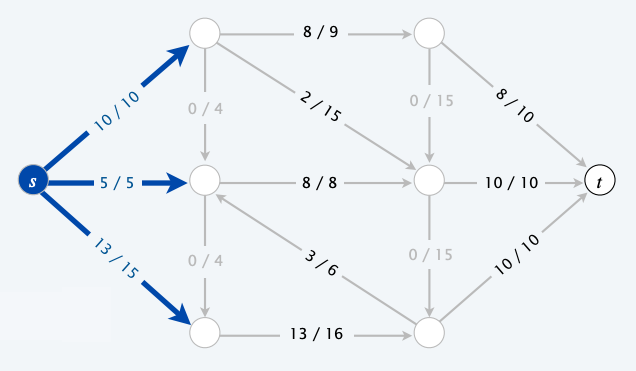
\includegraphics[width=0.7\linewidth]{images/worksheet_5_solution_3.png}
            \end{center}

            \bigskip

            Here, the maximum flow is $10 + 5 + 13 = 28$
        \end{itemize}

        \bigskip

        \item \textbf{Flow Network:}
        \begin{itemize}
            \item $G = (V,E)$ is a directed graph in which each edge $(u,v) \in E$
            has a nonnegative capacity $c(u,v) \geq 0$.
            \item Two vertices must exist: \textbf{source} s and \textbf{sink} t
            \item \textbf{path} from source $s$ to vertax $v$ to sink $t$ is represented by $s \rightsquigarrow v \rightsquigarrow t$

        \end{itemize}

        \bigskip

        \begin{center}
        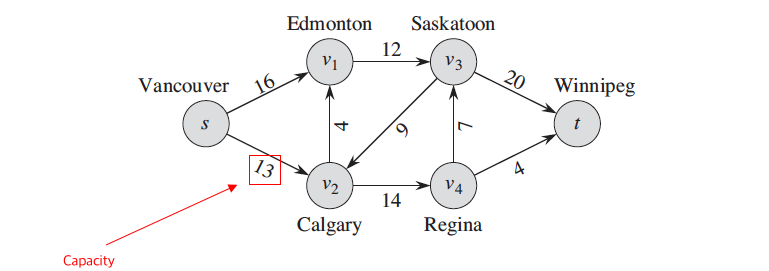
\includegraphics[width=0.9\linewidth]{images/worksheet_5_solution_1.png}
        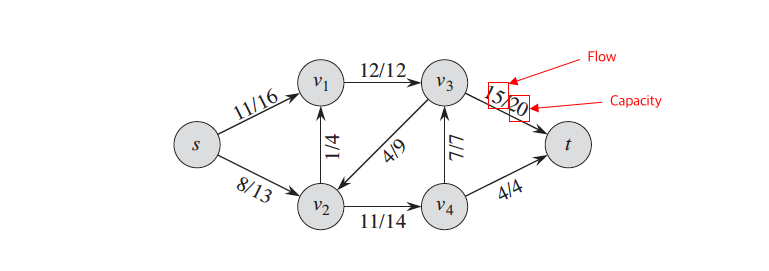
\includegraphics[width=0.9\linewidth]{images/worksheet_5_solution_2.png}
        \end{center}

        \item \textbf{Capacity:}

        \begin{itemize}
            \item Is a non-negative function $f: V \times V \to \mathbb{R}_{\geq 0}$
            \item Has \textbf{capacity constraint} where for all $u,v \in V$ $0 \leq f(u,v) \leq c(u,v)$

            \begin{itemize}
                \item Means flow cannot be above capacity constraint
            \end{itemize}
        \end{itemize}

        \item \textbf{Flow:}

        \begin{itemize}
            \item Is a real valued function $f: V \times V \to \mathbb{R}$ in $G$
            \item Satisfies \textbf{capacity constraint} (i.e for all $u,v \in V$, $0 \leq f(u,v) \leq c(u,v)$)
            \item Satisfies \textbf{flow conservation}

            \bigskip

            For all $u \in V - \{s,t\}$, we require

            \bigskip

            \begin{align}
            \sum\limits_{v \in V} f(v,u) = \sum\limits_{v \in V} f(u,v)
            \end{align}

            \bigskip

            \begin{itemize}
                \item Means flow into vertex $u$ is the same as flow going out of vertex $u$. $^{[1]}$
                \item $\sum\limits_{v \in V} f(u,v)$ means flow \underline{out of} vertex $u$
                \item $\sum\limits_{v \in V} f(v,u)$ means flow \underline{into} vertex $u$
                \item $v \in V$ in $\sum\limits_{v \in V} f(u,v)$ means all vertices that are an edge away from vertex $u$
            \end{itemize}

            \bigskip

            \underline{\textbf{Example:}}

            \begin{center}
            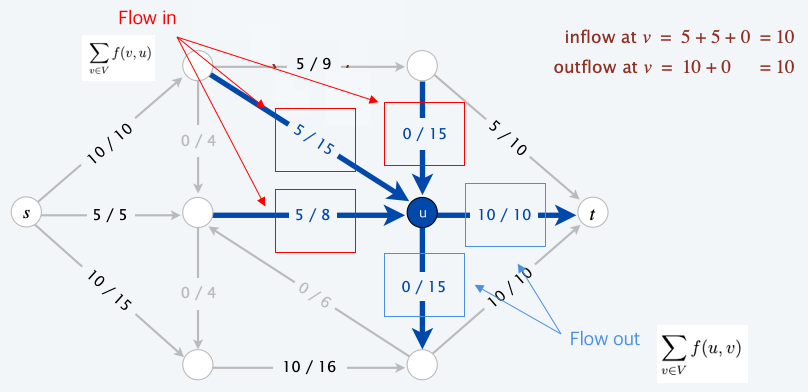
\includegraphics[width=0.9\linewidth]{images/worksheet_5_solution_4.png}
            \end{center}


        \end{itemize}
    \end{itemize}

    \bigskip

    \underline{\textbf{References}}

    \bigskip

    \begin{enumerate}[1)]
        \item Princeton University, Network Flow 1, \href{https://www.cs.princeton.edu/~wayne/kleinberg-tardos/pdf/07NetworkFlowI.pdf}{link}
    \end{enumerate}

    \item

    \bigskip

    I need to formulate the problem of determining whether both of professor Adam's two children can go to the same school
    as maximum-flow problem.

    \bigskip

    The problem statement tells us the following:

    \bigskip

    \begin{enumerate}[1.]
        \item There is 1 supersource (location of home)
        \item There is 1 sink (location of school)
        \item There are two sources ($s_1$ as child 1, $s_2$ as child 2)
        \item Edge $(u,v)$ has capacity of 0 or more (0 representing unavailable sidewalk, 1 for sidewalk with capacity of 1, 2 for street with capacity of 2 and so on)
        \item Each vertex represents corner of intersection, and two children can have their paths crossing here.
        \item Has flow of 2, 1 or 0 (1 is where one of the two children walking on the road. 0 is none.)
    \end{enumerate}

    \bigskip

    Here we are to find whether children must go on to a vertex and out to the same edge with the flow of 2,
    or determine whether there is only edge to school with capacity of 1 or less.

    \bigskip

    If none, then both children can safely go to school.

    \bigskip

    \begin{center}
    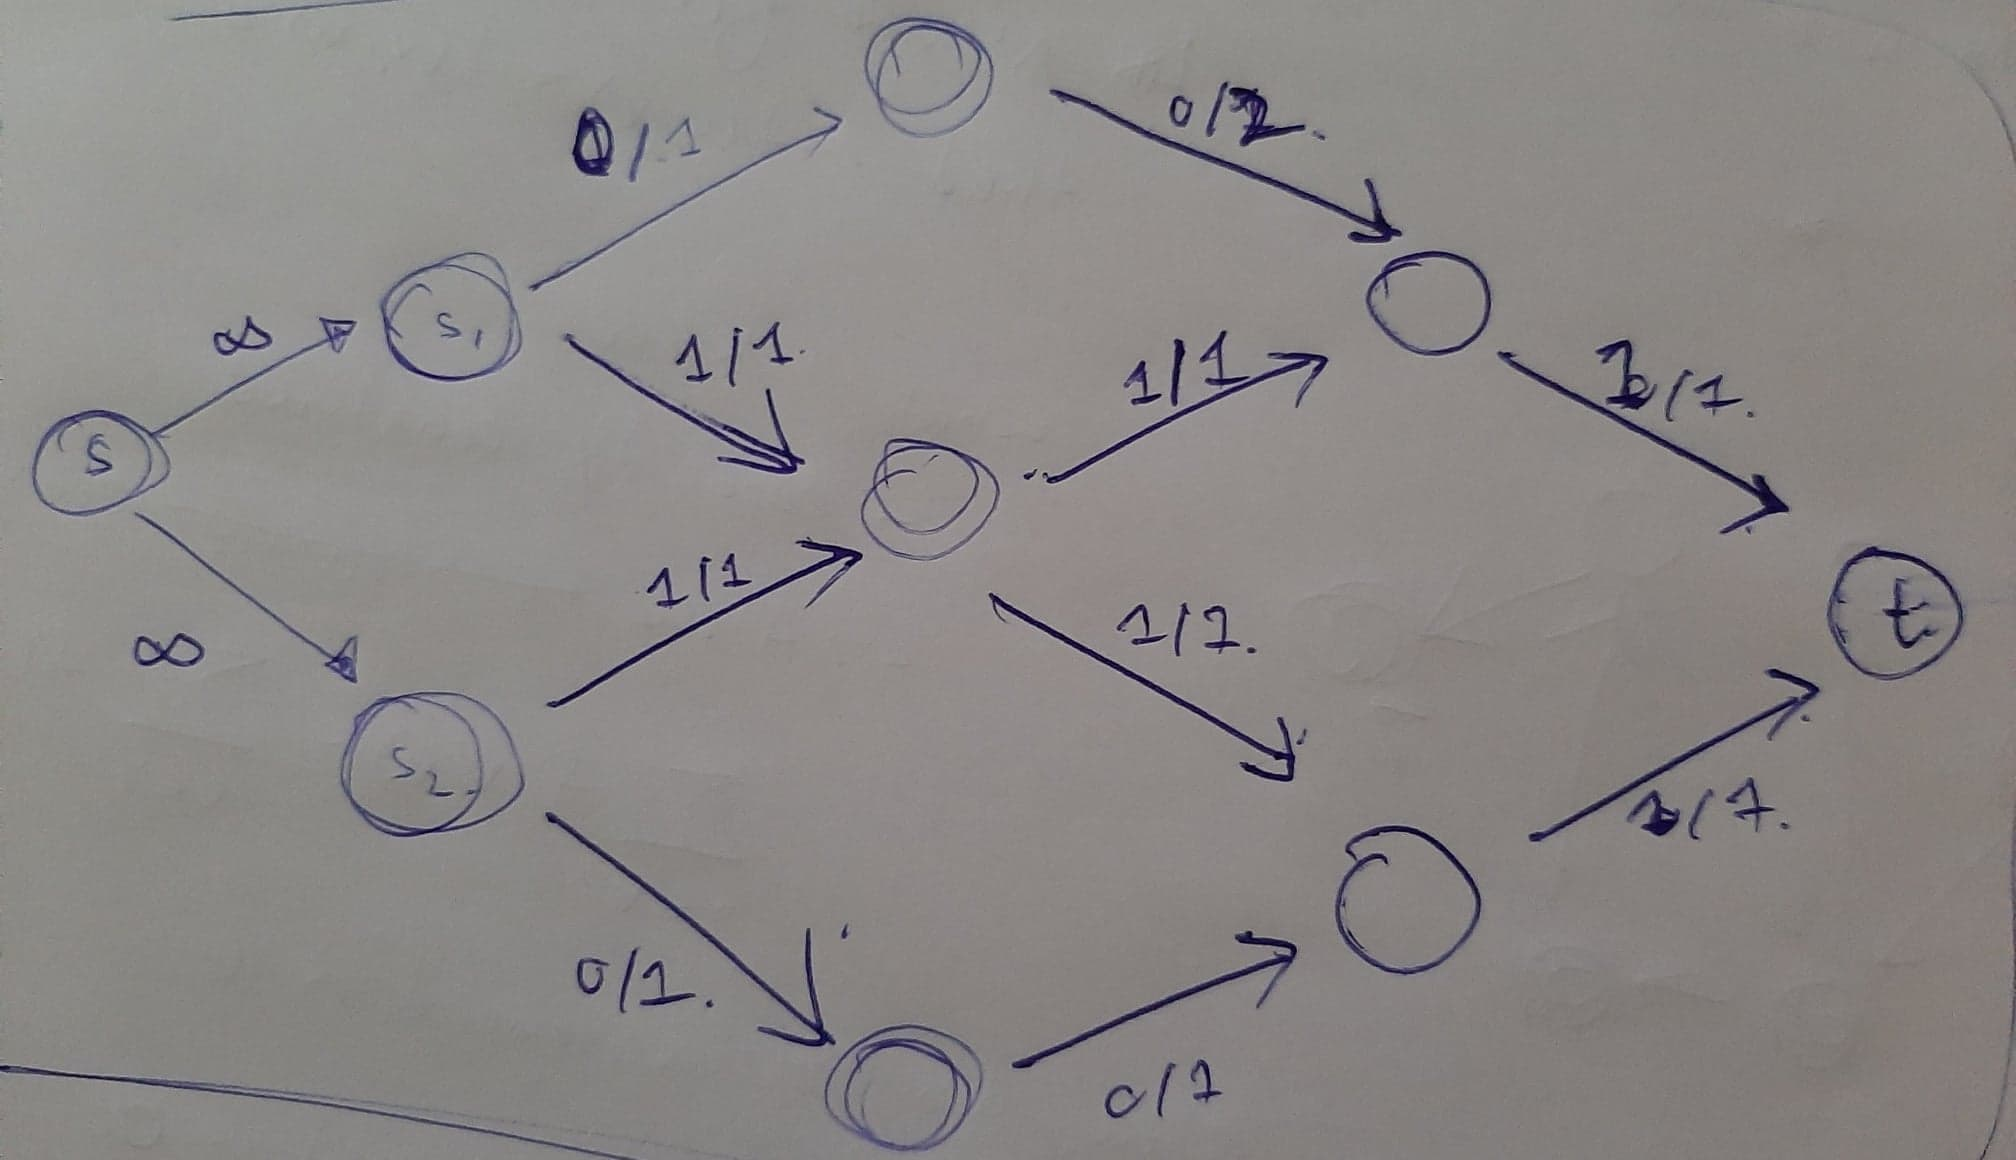
\includegraphics[width=0.7\linewidth]{images/worksheet_5_solution_7.jpg}
    \end{center}

    \bigskip

    % \underline{\textbf{Rough Works:}}

    % \bigskip

    % I need to formulate the problem of determining whether both of professor Adam's two children can go to the same school
    % as maximum-flow problem.

    % \bigskip

    % The problem statement tells us the following:

    % \bigskip

    % \begin{enumerate}[1.]
    %     \item There is 1 supersource (location of home)
    %     \item There is 1 sink (location of school)
    %     \item There are two sources ($s_1$ as child 1, $s_2$ as child 2)
    %     \item Edge $(u,v)$ has capacity of 0 or more (0 representing unavailable sidewalk, 1 for sidewalk with capacity of 1, 2 for street with capacity of 2 and so on)
    %     \item Each vertex represents corner of intersection, and two children can have their paths crossing here.
    %     \begin{itemize}
    %         \item But total inflow must equal total outflow (by flow conservation)
    %     \end{itemize}
    %     \item Has flow of 2, 1 or 0 (1 is where one of the two children walking on the road. 0 is none.)
    % \end{enumerate}

    % \bigskip

    % Here we are to find whether children must go on to a vertex and out to the same edge with the flow of 2,
    % or determine whether there is only edge to school with capacity of 1 or less.

    % \bigskip

    % If none, then both children can safely go to school.

    % \bigskip

    \underline{\textbf{Notes:}}

    \bigskip

    \begin{itemize}
        \item \textbf{Cross at a Corner}

        \begin{itemize}
            \item Means to walk across the street at a corner of the intersection.

            \bigskip

            \begin{center}
            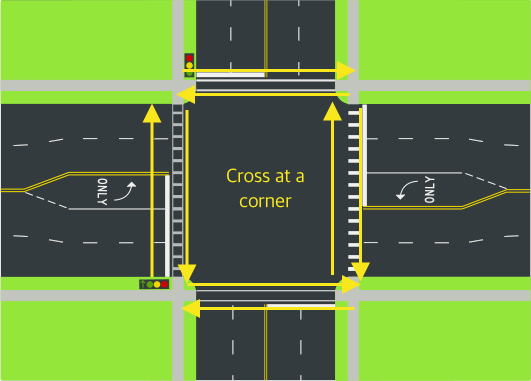
\includegraphics[width=0.7\linewidth]{images/worksheet_5_solution_5.png}
            \end{center}
        \end{itemize}

        \item \textbf{Multiple Sources and Sinks}

        \begin{itemize}
            \item Has edges $(s, s_i)$ where $i = 1 ... n$ and $(t_j, t)$ where $j = 1 ... n$
            with capacity of $\infty$
        \end{itemize}

        \bigskip

        \underline{\textbf{Example:}}

        \bigskip

        Lucky Puck Company having a set of $m$ factories $\{s_1, s_2, ..., s_m\}$, and
        a set of $n$ warehourses and $n$ warehouses $\{t_1, t_2, ..., t_n\}$

        \bigskip

        \begin{center}
        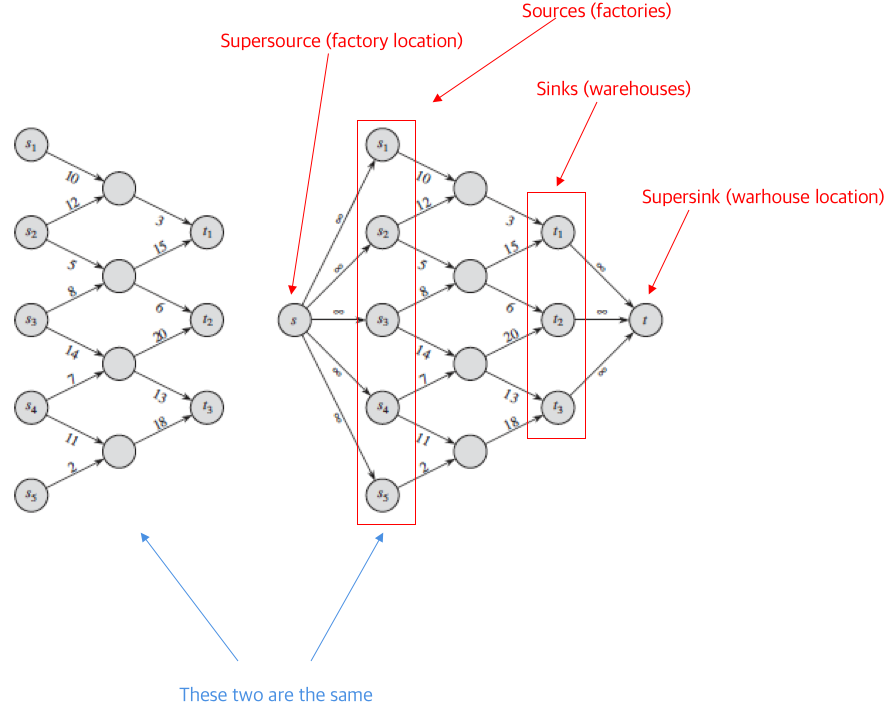
\includegraphics[width=0.9\linewidth]{images/worksheet_5_solution_6.png}
        \end{center}

    \end{itemize}

    \item

    \bigskip

    I need to show how to transform a flow network $G = (V,E)$ with vertex capacities
    into an equivalent flow network $G' = (V',E')$ without vertex capacities.

    \bigskip

    For each vertex capacities, change as follows.

    \begin{center}
    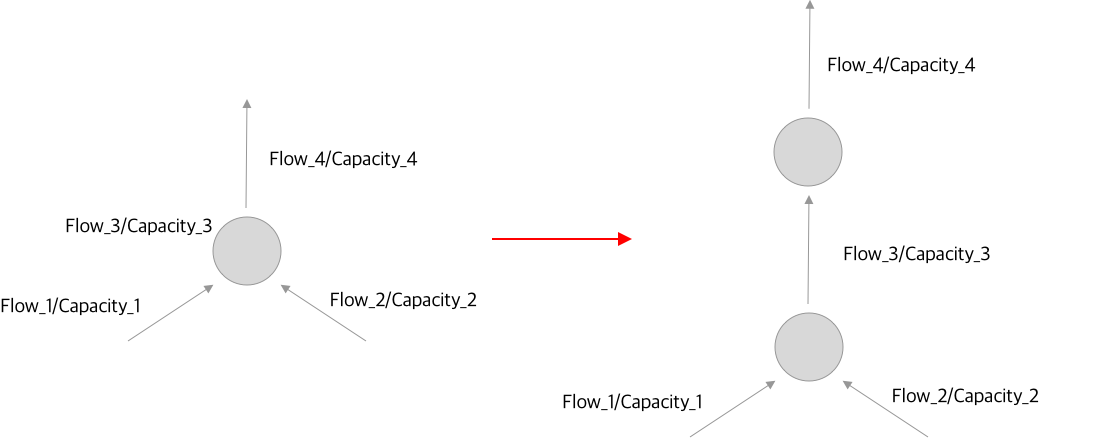
\includegraphics[width=0.9\linewidth]{images/worksheet_5_solution_8.png}
    \end{center}

    \bigskip

    After transformation, there will be $m$ more edges and verticies, where $m$
    represents the number of vertex capacities in $G$.

    \bigskip

    \underline{\textbf{Notes:}}

    \bigskip

    \begin{itemize}
        \item \textbf{Vertex Capacities}
        \begin{itemize}
            \item Each vertex $v$ has limit $l(v)$ on how much flow can pass through $v$
        \end{itemize}
    \end{itemize}

    \item

    \bigskip

    I need to show how to convert the problem of finding a flow $f$ that obeys the
    constraints into the problem of finding a maximum flow in a single
    source, single-sink flow network

    \bigskip

    The steps are as follows:

    \bigskip

    \begin{itemize}
        \item Combine all sources $s_i$ into a single source $s$
        \item Combine all sinks $t_j$ into a single sink $t$
        \item Connect source $s$ to each adjacent vertex $v$ with edge weight $\sum\limits_{i} f(s_i, v) = p_i$

        \begin{itemize}
            \item The total edge weight from $s$ should be $\sum\limits_{i} p_i$
        \end{itemize}

        \item Connect each adjacent vertex $v$ of t to $t$ with edge weight $\sum\limits_{j} f(v,t_j) = q_j$

        \begin{itemize}
            \item The total edge weight to $t$ should be $\sum\limits_{j} q_j$
        \end{itemize}


        \item Find a simple path from $s$ to $t$ with the maximum amount of total flow
    \end{itemize}

    \begin{center}
    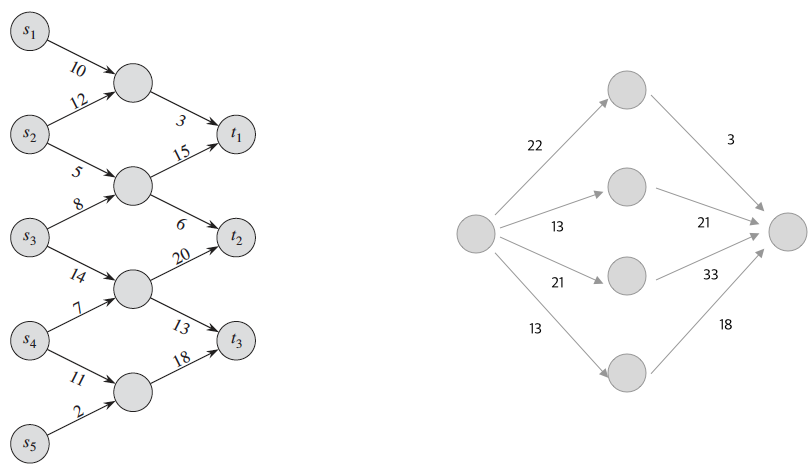
\includegraphics[width=0.9\linewidth]{images/worksheet_5_solution_16.png}
    \end{center}

    \bigskip

    \begin{mdframed}
        \underline{\textbf{Correct Solution:}}


        I need to show how to convert the problem of finding a flow $f$ that obeys the
        constraints into the problem of finding a maximum flow in a single
        source, single-sink flow network

        \bigskip

        The steps are as follows:

        \bigskip

        \begin{itemize}
            \item Combine all sources $s_i$ into a single source $s$
            \item Combine all sinks $t_j$ into a single sink $t$
            \item Connect source $s$ to each adjacent vertex $v$ with edge weight $\sum\limits_{i} f(s_i, v) = p_i$

            \begin{itemize}
                \item The total edge weight from $s$ should be $\sum\limits_{i} p_i$
            \end{itemize}

            \item Connect each adjacent vertex $v$ of t to $t$ with edge weight $\sum\limits_{j} f(v,t_j) = q_j$

            \begin{itemize}
                \item The total edge weight to $t$ should be $\sum\limits_{j} q_j$
            \end{itemize}


            \item Find a simple path from $s$ to $t$ with the maximum amount of total flow
        \end{itemize}

        \color{red}\underline{\textbf{Example}}\color{black}

        \begin{center}
        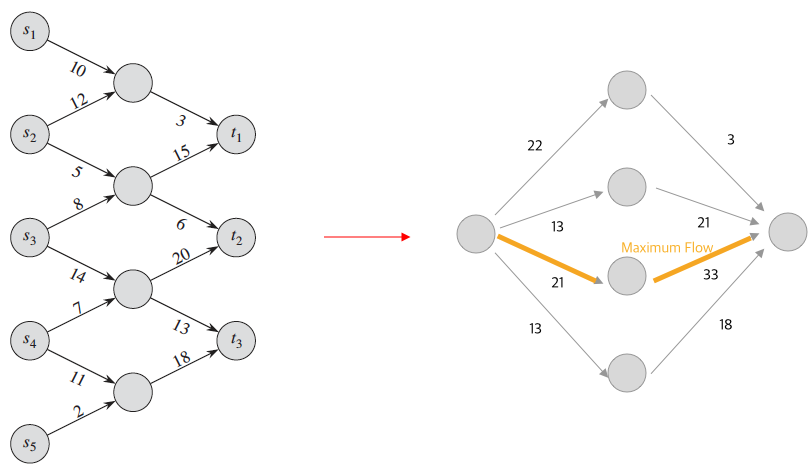
\includegraphics[width=0.9\linewidth]{images/worksheet_5_solution_17.png}
        \end{center}

    \end{mdframed}

    \bigskip

    % \underline{\textbf{Rough Works:}}

    % \bigskip

    % I need to show how to convert the problem of finding a flow $f$ that obeys the
    % constraints into the problem of finding a maximum flow in a single
    % source, single-sink flow network

    % \bigskip

    % The steps are as follows:

    % \bigskip

    % \begin{itemize}
    %     \item Combine all sources $s_i$ into a single source $s$
    %     \item Combine all sinks $t_j$ into a single sink $t$
    %     \item Connect source $s$ to each adjacent vertex $v$ with edge weight $\sum\limits_{i} f(s_i, v) = p_i$

    %     \begin{itemize}
    %         \item The total edge weight from $s$ should be $\sum\limits_{i} p_i$
    %     \end{itemize}

    %     \item Connect each adjacent vertex $v$ of t to $t$ with edge weight $\sum\limits_{j} f(v,t_j) = q_j$

    %     \begin{itemize}
    %         \item The total edge weight to $t$ should be $\sum\limits_{j} q_j$
    %     \end{itemize}


    %     \item Find a simple path from $s$ to $t$ with the maximum amount of total flow
    % \end{itemize}

    % \begin{center}
    % 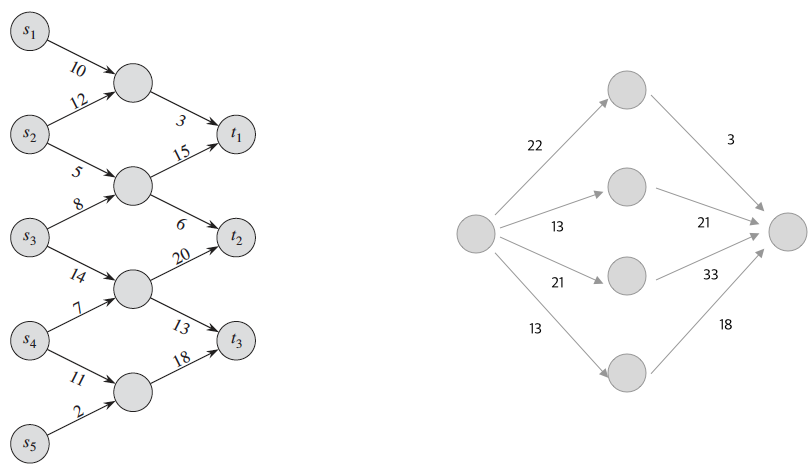
\includegraphics[width=0.9\linewidth]{images/worksheet_5_solution_16.png}
    % \end{center}


    % \bigskip

    \underline{\textbf{Notes:}}

    \bigskip

    \begin{itemize}
        \item \textbf{Ford-Fulkerson Method}

        \begin{itemize}
            \item Is a greedy algorithm that solves the maximum-flow problem
            \begin{itemize}
                \item Determines maximum flow from start vertex to sink vertex in a graph
            \end{itemize}
            \item Called method (not algorithm) because several different implementations
            with different running time is used
        \end{itemize}

        \begin{center}
        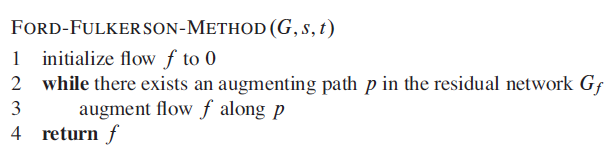
\includegraphics[width=0.9\linewidth]{images/worksheet_5_solution_9.png}
        \end{center}

        \item \textbf{Residual Network}
        \begin{itemize}
            \item Indicates how muh more flow is allowed in each edge in the network graph $^{[1]}$
            \item Consists of edges with capacities that represents how we can change the flow on edges of $G$.
            \item Provides roadmap for adding flow to the original flow network
        \end{itemize}

        \bigskip

        \begin{center}
        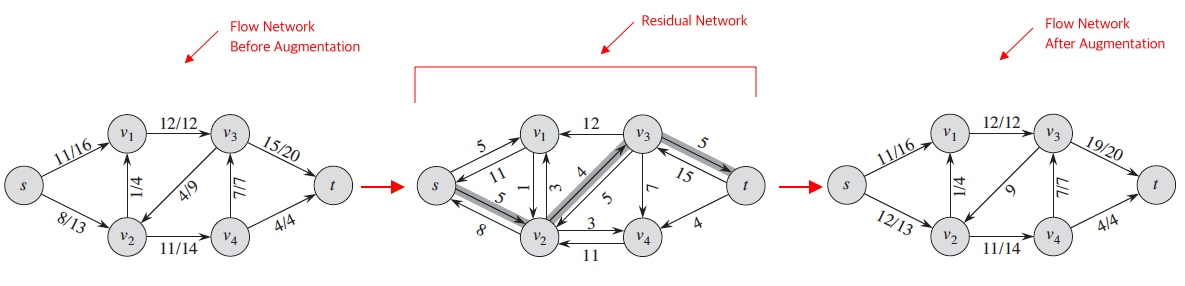
\includegraphics[width=\linewidth]{images/worksheet_5_solution_12.png}
        \end{center}

        \bigskip

        \underline{\textbf{Steps}}

        \bigskip

        \begin{enumerate}[1)]
            \item \textbf{$Flow = Capacity$:} Opposite arrow

            \begin{center}
            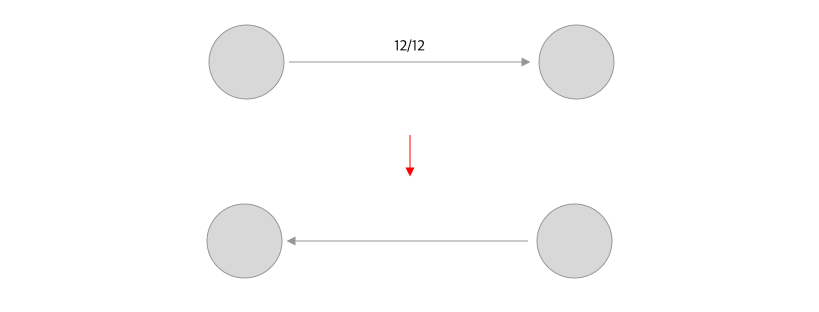
\includegraphics[width=0.8\linewidth]{images/worksheet_5_solution_10.png}
            \end{center}

            \item \textbf{$Flow < Capacity$:}

            \begin{itemize}
                \item \textbf{$Flow$:} Oppisite Arrow
                \item \textbf{$Capacity - Flow$:} Current Arrow
            \end{itemize}

            \begin{center}
            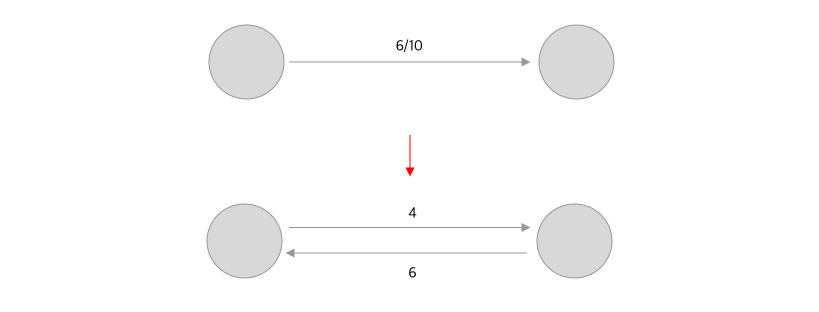
\includegraphics[width=0.8\linewidth]{images/worksheet_5_solution_11.png}
            \end{center}
        \end{enumerate}

        \bigskip

        \item \textbf{Augmenting Path}

        \begin{itemize}
            \item Is a path from source S to sink T where you can increase the amount of flow
            \item Is a path that doesn't contain cycle (simple path) $^{[2]}$

            \begin{center}
            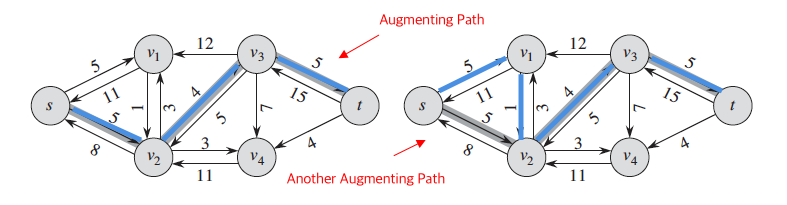
\includegraphics[width=\linewidth]{images/worksheet_5_solution_13.png}
            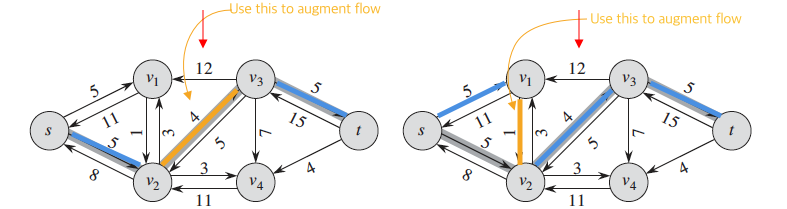
\includegraphics[width=\linewidth]{images/worksheet_5_solution_14.png}
            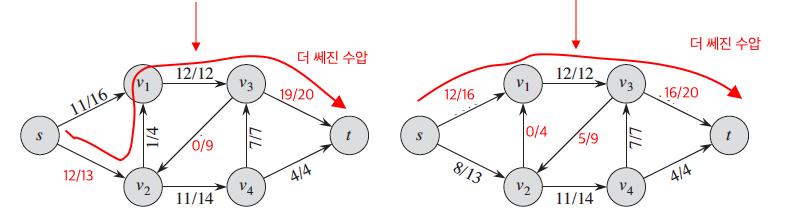
\includegraphics[width=\linewidth]{images/worksheet_5_solution_15.png}
            \end{center}

            \item Edge $(u,v)$ on simple path on an augmenting path can be increased
            by upto $c_f(u,v)$ withhout violating the capacity constraint
        \end{itemize}

        \item \textbf{Augmentation}

        \begin{itemize}
            \item 한국어로 '불필요한 수압 decrease 해서 앞으로 가는 수압 더 쎄게 만들기'
            \item Is symbolized by $f \uparrow f'$

            \begin{itemize}
                \item $f$ is a flow in $G$
                \item $f'$ is a flow in the residual network $G_f$
            \end{itemize}
        \end{itemize}

    \end{itemize}

    \bigskip

    \underline{\textbf{References}}

    \bigskip

    \begin{enumerate}[1)]
        \item Hacker Earth, Maximum Flow, \href{https://www.hackerearth.com/practice/algorithms/graphs/maximum-flow/tutorial/}{link}
        \item Stack Overflow, What Exactly Is Augmentation Path, \href{https://stackoverflow.com/questions/10397118/what-exactly-is-augmenting-path}{link}
    \end{enumerate}

    \item

    \bigskip

    \underline{\textbf{Rough Works:}}

    \bigskip

    I need to show if the augmented flow of $f$ and $f'$ $\in G$ and satisfy the
    flow conservation property and capacity constraint.

    \bigskip

    \begin{itemize}
        \item Proving that $f \uparrow f'$ satisfies the flow conservation property

        \begin{enumerate}[1)]
            \item
        \end{enumerate}

        \item Proving that $f \uparrow f'$ satisfies the capacity constraint
    \end{itemize}

    \bigskip

    \underline{\textbf{Notes:}}

    \bigskip

    \begin{itemize}
        \item I need clarification from professor about the meaning of $f' \in G$.
        Is $f'$ a flow from flow network or residual network?
        \item I feel I am struggling because I am jumping to solution without understanding the problem
        \item Noticed that a solution in University of Texas really elaborated on $f \uparrow f'(u,v)$
        before moving onto strategizing and constructing a solution

        \begin{center}
        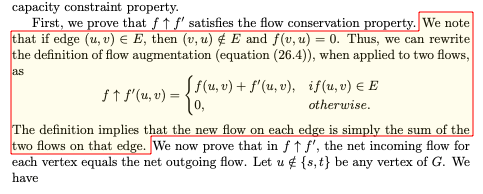
\includegraphics[width=0.8\linewidth]{images/worksheet_5_solution_18.png}
        \end{center}

        \item \textbf{Flow Network (cont'd)} [Important!]

        \begin{itemize}
            \item Flow network requires that

            \begin{enumerate}[1)]
                \item $G = (V,E)$ is a directed graph
                \item each edge $(u,v) \in E$ has a non-negative capacity $c(u,v) \geq 0$
                \item \color{red}\ul{If $E$ contains an edge $(u,v)$, then there is no edge $(v,u)$ in the reverse direction (no anti-parallel edge)}\color{black}
            \end{enumerate}
        \end{itemize}

        \item \textbf{Augmentation (cont'd)}

        \begin{itemize}
            \item Augmentation of flow $f$ by $f'$ or $f \uparrow f'$ is a function
            $V \times V \to \mathbb{R}$ is defined by


            \begin{align}
                (f \uparrow f')(u,v) &= \begin{cases}
                    f(u,v) + f'(u,v) - f'(v,u) & [\text{If $(u,v) \in E$}]\\
                    0 & [\text{Otherwise}]
                \end{cases}
            \end{align}
        \end{itemize}

        \item \textbf{Proof of flow conservation for $f \uparrow f'$ when $f \in G$ and $f' \in G_f$}
        \setcounter{equation}{0}
        \bigskip

        Let $G = (V,E)$ be a flow network with sources $s$ and sink $t$. Let $f$
        be a flow in $G$. Let $G_f$ be a residual network of $G$ induced by $f$ and let $f'$ be
        a flow in $G_f$. We note that if $(u,v) \in E$, then $(v,u) \notin E$ and $f(v,u) = 0$. Thus,
        the definition


        \begin{align}
            (f \uparrow f')(u,v) &= \begin{cases}
                f(u,v) + f'(u,v) - f'(v,u) & [\text{If $(u,v) \in E$}]\\
                0 & [\text{Otherwise}]
            \end{cases}
        \end{align}

        \bigskip

        implies that the augmented flow $f \uparrow f'(u,v)$ on edge $(u,v)$ is the
        sum of flow $f(u,v)$ in flow network $G$ and flow $f'(u,v)$ minus its antiparallel
        flow $-f'(v,u)$ in residual flow network $G'$.

        \bigskip

        We now prove that the augmented flow satisfies flow conservation. That is,

        \begin{align}
        \sum\limits_{v \in V} f \uparrow f' (u,v) = \sum\limits_{v \in V} f \uparrow f' (v,u)
        \end{align}.

        \bigskip

        And indeed we have

        \begin{align}
            \sum\limits_{v \in V} f \uparrow f' (u,v) &= \sum\limits_{v \in V} f(u,v) + f'(u,v) - f'(v,u) & [\text{By augmentation def.}]\\
            &= \sum\limits_{v \in V} f(u,v) + \sum\limits_{v \in V} f'(u,v) - \sum\limits_{v \in V} f'(v,u)\\
            &= \sum\limits_{v \in V} f(v,u) + \sum\limits_{v \in V} f'(v,u) - \sum\limits_{v \in V} f'(u,v) & [\text{By flow conserv. of $f$ and $f'$}]\\
            &= \sum\limits_{v \in V} f(v,u) + f'(v,u) - f'(u,v)\\
            &= \sum\limits_{v \in V} f \uparrow f' (v,u)
        \end{align}


        \bigskip

        \begin{itemize}
            \item \color{red}Flow in residual network also obey flow conservation\color{black}
        \end{itemize}

        \item \textbf{Proof of capacity constraint for $f \uparrow f'$ when $f \in G$ and $f' \in G_f$}
    \end{itemize}

\end{enumerate}

\end{document}